\section{Artifact map}

The paper is generated from current local artifacts rather than hand-entered
plots.  The figure-generation script is
\path{scripts/plot_paper_b.py}.  It writes figures to
\path{paper_b/figures/} and a JSON snapshot to
\path{paper_b/generated_results/result_snapshot.json}.

\begin{table}[H]
\centering
\footnotesize
\caption{Primary local result sources used by this paper.}
\begin{tabularx}{\linewidth}{lY}
\toprule
Claim & Local source\\
\midrule
PushT checkpointed downstream use
  & \path{outputs/pusht_checkpointed_downstream_use_v1/summary.json}\\
PointMaze carrier grid
  & \path{outputs/dinowm_pointmaze_wave3/formal/carrier_summary.json}\\
PointMaze external use
  & \path{outputs/dinowm_pointmaze_wave3/formal/external_use_summary.json}\\
Wall PCA-logistic confirmation
  & \path{outputs/dinowm_wall_audit_v1/stage_h_logistic_readout/summary.json}\\
Wall ridge screen
  & \path{outputs/dinowm_wall_audit_v1/stage_h_carriers/summary.json}\\
OGBench admission bridge
  & \path{outputs/ogbench_mesmem_admission_v1/summary_all.json}\\
OGBench feature-host capacity
  & \path{outputs/ogbench_feature_host_stage_v1/summary.json}\\
OGBench native-use success
  & \path{outputs/ogbench_native_use_stage_v1/summary.json}\\
OGBench repaired all-env native-use success
  & \path{outputs/native_use_repaired_combined_v1/summary.json}\\
Final non-manual OGBench patch-set JEPA
  & \path{outputs/random_patchset_view_color_jepa_final_v1/summary.json}\\
\bottomrule
\end{tabularx}
\end{table}

\section{Generated all-env native-use repair monitor}
\label{app:native-use-repaired-auto}

This section is generated from \path{outputs/native_use_repaired_combined_v1/summary.json}.  It records the fixed-controller native-use sweep after the multi-object controller repair.  Rows without an audited local controller, or rows whose oracle-label controller gate fails, remain unscored scope limits.

\begin{table}[H]
\centering
\footnotesize
\setlength{\tabcolsep}{4.2pt}
\renewcommand{\arraystretch}{1.08}
\caption{Repaired all-env fixed-controller native-use summary.  Full memory is the ME-JEPA memory-selected target; control is the stronger of recent-only and random selection, averaged over the listed rows.  The sweep scores 24/36 env-age rows, with mean full success 0.952, worst scored full success 0.828, and mean full-minus-control lifts 0.714 over recent-only and 0.708 over random.}
\label{tab:native-use-repaired-allenv}
\begin{tabular}{lccccc}
\toprule
Group & Rows & Full & Control & Oracle & Status\\
\midrule
PointMaze non-teleport & 9 & 0.993 & 0.252 & 1.000 & scored\\
Cube-single & 3 & 1.000 & 0.246 & 1.000 & scored\\
Cube-double & 3 & 0.944 & 0.281 & 0.944 & repaired\\
Cube-triple & 3 & 0.911 & 0.222 & 0.911 & repaired\\
Puzzle-3x3 & 3 & 0.928 & 0.254 & 1.000 & scored\\
Scene & 3 & 0.854 & 0.239 & 0.903 & repaired\\
PointMaze-teleport & 0 & \NA & \NA & 0.608--0.658 & gate failed\\
Ant/Humanoid locomotion & 0 & \NA & \NA & \NA & no local controller\\
\bottomrule
\end{tabular}
\end{table}


\section{Generated non-manual breadth monitor}
\label{app:nonmanual-breadth-auto}

This section is generated automatically by the overnight controller.  It is
included to remove ambiguity between clean paper-level claims and broader
stress tests.  A row marked mixed is not promoted to a main-text claim; it
identifies an environment-age setting that requires confirmation or a design
change.

\paragraph{Generation status.} Overnight sequence completed. Last update: 2026-07-17T02:57:48.

\paragraph{Random patch-set breadth wave.}
This generated block reports 13/21 environment-age rows passing the
registered non-manual gate. Mixed rows are treated as stress-test limits or
confirmation targets, not as headline wins.

\begin{figure}[!tbp]
\centering
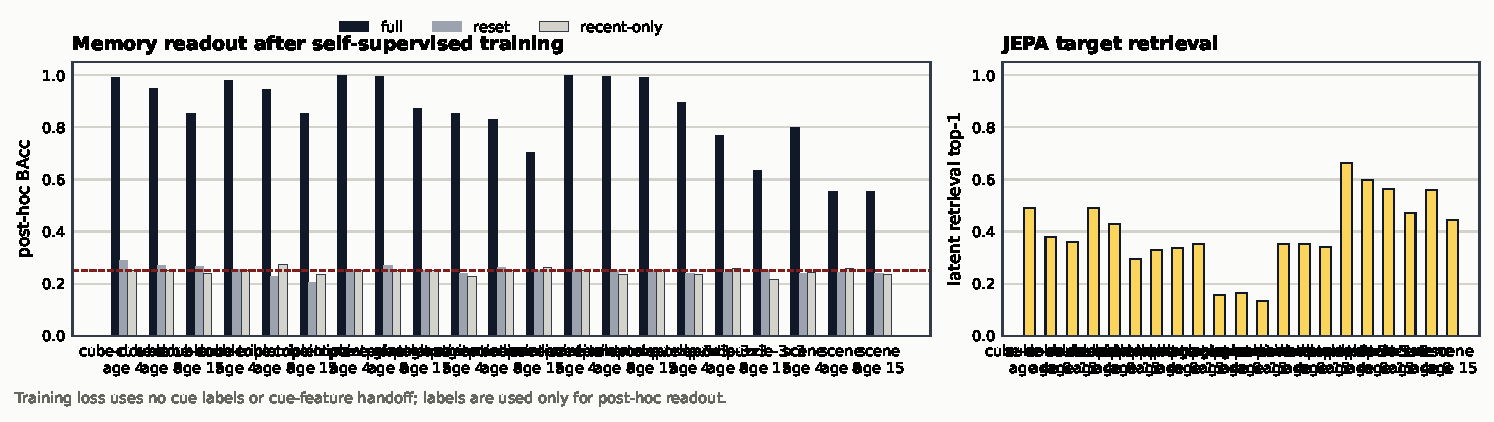
\includegraphics[width=\linewidth]{figures/fig_b_nonmanual_breadth_auto.pdf}
\caption{Generated non-manual breadth plot for Random patch-set breadth wave.}
\end{figure}

\begin{table}[!tbp]
\centering
\scriptsize
\setlength{\tabcolsep}{3.5pt}
\renewcommand{\arraystretch}{1.05}
\caption{Generated non-manual breadth table for Random patch-set breadth wave.}
\begin{tabular}{lccccccl}
\toprule
Deck & Age & Seeds & Pass & Full & Reset & Recent & Status\\
\midrule
cube-double-play-v0 & 4 & 3 & 3/3 & 0.991 & 0.289 & 0.250 & \textsc{pass}\\
cube-double-play-v0 & 8 & 3 & 2/3 & 0.949 & 0.270 & 0.249 & \textsc{mixed}\\
cube-double-play-v0 & 15 & 3 & 3/3 & 0.854 & 0.266 & 0.238 & \textsc{pass}\\
cube-triple-play-v0 & 4 & 3 & 3/3 & 0.981 & 0.255 & 0.251 & \textsc{pass}\\
cube-triple-play-v0 & 8 & 3 & 3/3 & 0.947 & 0.228 & 0.275 & \textsc{pass}\\
cube-triple-play-v0 & 15 & 3 & 3/3 & 0.852 & 0.206 & 0.237 & \textsc{pass}\\
pointmaze-giant-navigate-v0 & 4 & 3 & 3/3 & 1.000 & 0.250 & 0.250 & \textsc{pass}\\
pointmaze-giant-navigate-v0 & 8 & 3 & 3/3 & 0.993 & 0.271 & 0.250 & \textsc{pass}\\
pointmaze-giant-navigate-v0 & 15 & 3 & 3/3 & 0.874 & 0.250 & 0.250 & \textsc{pass}\\
pointmaze-medium-navigate-v0 & 4 & 3 & 3/3 & 0.853 & 0.240 & 0.228 & \textsc{pass}\\
pointmaze-medium-navigate-v0 & 8 & 3 & 2/3 & 0.830 & 0.262 & 0.251 & \textsc{mixed}\\
pointmaze-medium-navigate-v0 & 15 & 3 & 1/3 & 0.702 & 0.249 & 0.263 & \textsc{mixed}\\
pointmaze-teleport-navigate-v0 & 4 & 3 & 3/3 & 1.000 & 0.250 & 0.249 & \textsc{pass}\\
pointmaze-teleport-navigate-v0 & 8 & 3 & 3/3 & 0.996 & 0.250 & 0.235 & \textsc{pass}\\
pointmaze-teleport-navigate-v0 & 15 & 3 & 3/3 & 0.993 & 0.250 & 0.250 & \textsc{pass}\\
puzzle-3x3-play-v0 & 4 & 3 & 3/3 & 0.896 & 0.238 & 0.234 & \textsc{pass}\\
puzzle-3x3-play-v0 & 8 & 3 & 1/3 & 0.770 & 0.242 & 0.259 & \textsc{mixed}\\
puzzle-3x3-play-v0 & 15 & 3 & 1/3 & 0.636 & 0.250 & 0.218 & \textsc{mixed}\\
scene-play-v0 & 4 & 3 & 2/3 & 0.799 & 0.238 & 0.243 & \textsc{mixed}\\
scene-play-v0 & 8 & 3 & 0/3 & 0.553 & 0.243 & 0.257 & \textsc{mixed}\\
scene-play-v0 & 15 & 3 & 0/3 & 0.552 & 0.239 & 0.235 & \textsc{mixed}\\
\bottomrule
\end{tabular}
\end{table}

\paragraph{Large-bank confirmation.}
This generated block reports 8/12 environment-age rows passing the
registered non-manual gate. Mixed rows are treated as stress-test limits or
confirmation targets, not as headline wins.

\begin{figure}[!tbp]
\centering
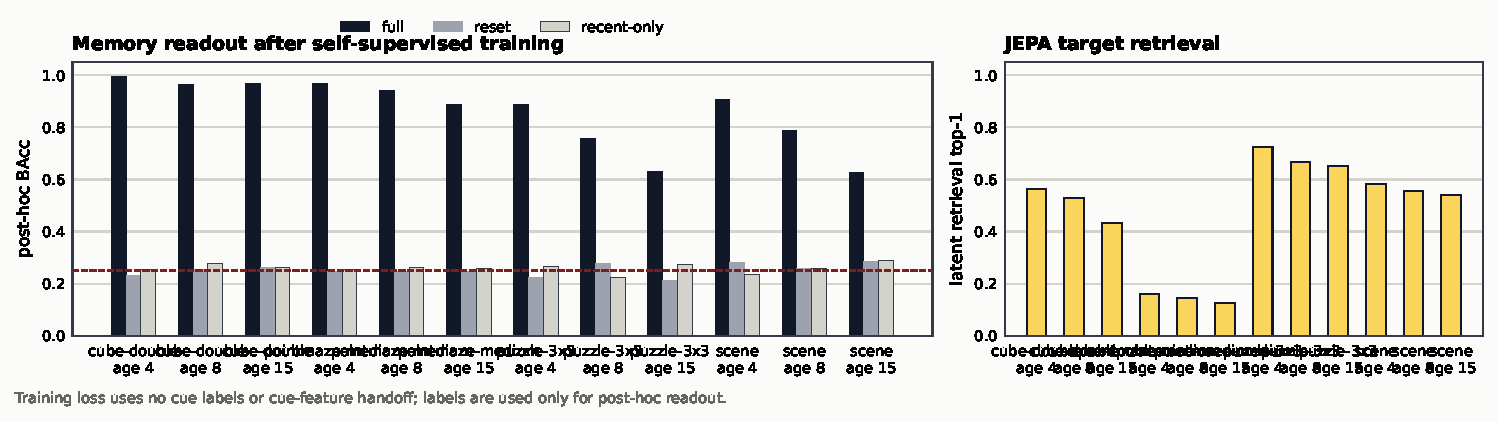
\includegraphics[width=\linewidth]{figures/fig_b_nonmanual_breadth_confirm_auto.pdf}
\caption{Generated non-manual breadth plot for Large-bank confirmation.}
\end{figure}

\begin{table}[!tbp]
\centering
\scriptsize
\setlength{\tabcolsep}{3.5pt}
\renewcommand{\arraystretch}{1.05}
\caption{Generated non-manual breadth table for Large-bank confirmation.}
\begin{tabular}{lccccccl}
\toprule
Deck & Age & Seeds & Pass & Full & Reset & Recent & Status\\
\midrule
cube-double-play-v0 & 4 & 3 & 3/3 & 0.995 & 0.233 & 0.255 & \textsc{pass}\\
cube-double-play-v0 & 8 & 3 & 3/3 & 0.964 & 0.253 & 0.277 & \textsc{pass}\\
cube-double-play-v0 & 15 & 3 & 3/3 & 0.969 & 0.264 & 0.263 & \textsc{pass}\\
pointmaze-medium-navigate-v0 & 4 & 3 & 3/3 & 0.968 & 0.248 & 0.255 & \textsc{pass}\\
pointmaze-medium-navigate-v0 & 8 & 3 & 3/3 & 0.941 & 0.249 & 0.263 & \textsc{pass}\\
pointmaze-medium-navigate-v0 & 15 & 3 & 3/3 & 0.888 & 0.246 & 0.260 & \textsc{pass}\\
puzzle-3x3-play-v0 & 4 & 3 & 3/3 & 0.888 & 0.225 & 0.265 & \textsc{pass}\\
puzzle-3x3-play-v0 & 8 & 3 & 1/3 & 0.757 & 0.277 & 0.225 & \textsc{mixed}\\
puzzle-3x3-play-v0 & 15 & 3 & 0/3 & 0.632 & 0.212 & 0.272 & \textsc{mixed}\\
scene-play-v0 & 4 & 3 & 3/3 & 0.906 & 0.282 & 0.237 & \textsc{pass}\\
scene-play-v0 & 8 & 3 & 1/3 & 0.787 & 0.260 & 0.257 & \textsc{mixed}\\
scene-play-v0 & 15 & 3 & 0/3 & 0.626 & 0.286 & 0.288 & \textsc{mixed}\\
\bottomrule
\end{tabular}
\end{table}

\paragraph{antmaze-large-navigate-v0.}
This generated block reports 3/3 environment-age rows passing the
registered non-manual gate. Mixed rows are treated as stress-test limits or
confirmation targets, not as headline wins.

\begin{figure}[!tbp]
\centering
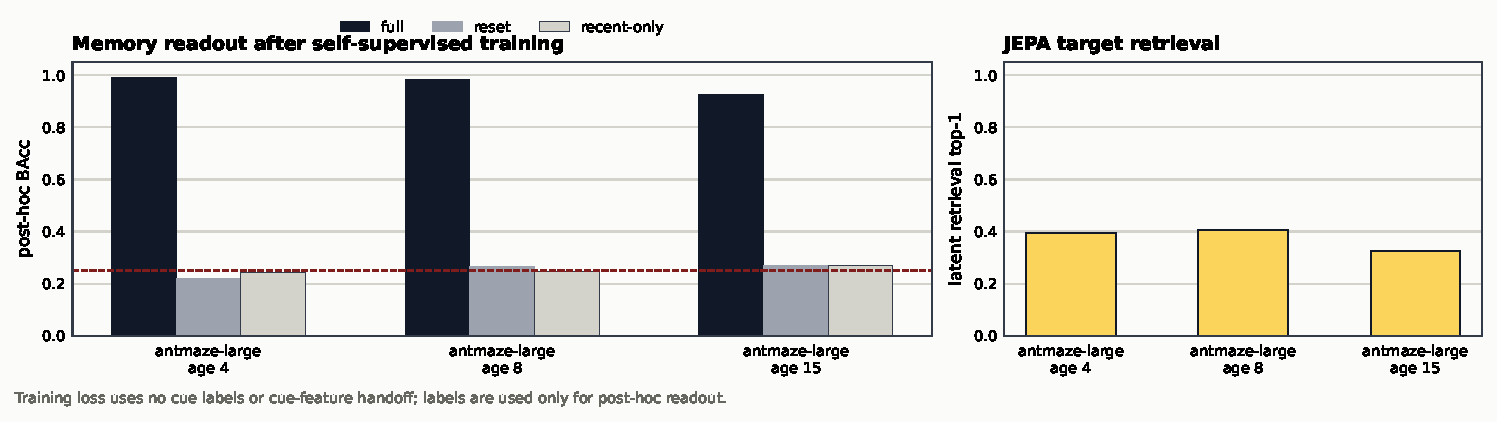
\includegraphics[width=\linewidth]{figures/fig_b_nonmanual_extra_antmaze_large_navigate_v0.pdf}
\caption{Generated non-manual breadth plot for antmaze-large-navigate-v0.}
\end{figure}

\begin{table}[!tbp]
\centering
\scriptsize
\setlength{\tabcolsep}{3.5pt}
\renewcommand{\arraystretch}{1.05}
\caption{Generated non-manual breadth table for antmaze-large-navigate-v0.}
\begin{tabular}{lccccccl}
\toprule
Deck & Age & Seeds & Pass & Full & Reset & Recent & Status\\
\midrule
antmaze-large-navigate-v0 & 4 & 3 & 3/3 & 0.992 & 0.220 & 0.243 & \textsc{pass}\\
antmaze-large-navigate-v0 & 8 & 3 & 3/3 & 0.985 & 0.264 & 0.245 & \textsc{pass}\\
antmaze-large-navigate-v0 & 15 & 3 & 3/3 & 0.925 & 0.268 & 0.271 & \textsc{pass}\\
\bottomrule
\end{tabular}
\end{table}

\paragraph{antmaze-giant-navigate-v0.}
This generated block reports 3/3 environment-age rows passing the
registered non-manual gate. Mixed rows are treated as stress-test limits or
confirmation targets, not as headline wins.

\begin{figure}[!tbp]
\centering
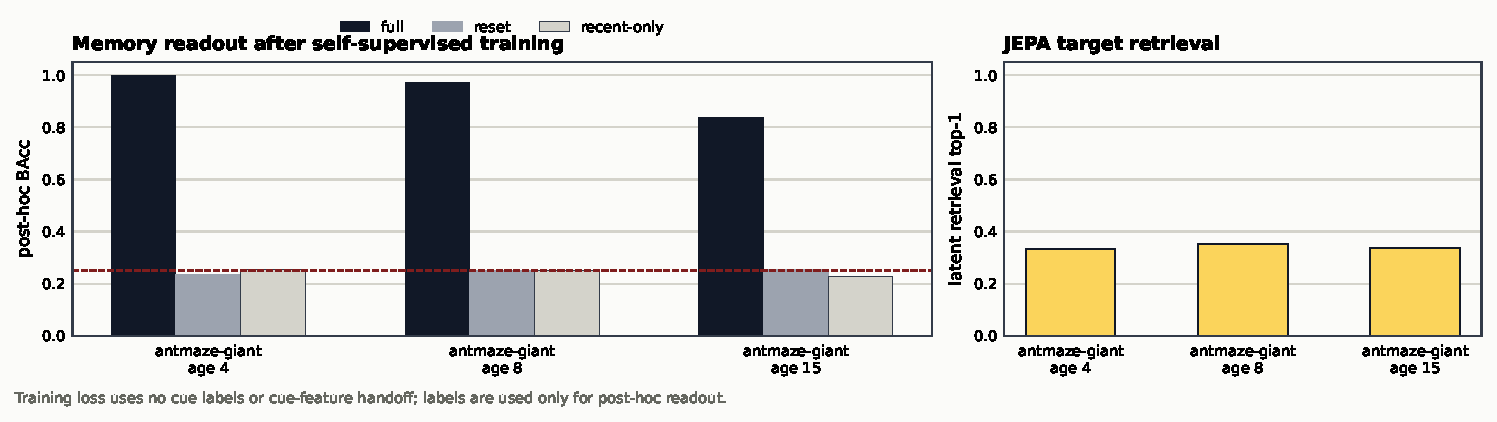
\includegraphics[width=\linewidth]{figures/fig_b_nonmanual_extra_antmaze_giant_navigate_v0.pdf}
\caption{Generated non-manual breadth plot for antmaze-giant-navigate-v0.}
\end{figure}

\begin{table}[!tbp]
\centering
\scriptsize
\setlength{\tabcolsep}{3.5pt}
\renewcommand{\arraystretch}{1.05}
\caption{Generated non-manual breadth table for antmaze-giant-navigate-v0.}
\begin{tabular}{lccccccl}
\toprule
Deck & Age & Seeds & Pass & Full & Reset & Recent & Status\\
\midrule
antmaze-giant-navigate-v0 & 4 & 3 & 3/3 & 1.000 & 0.235 & 0.254 & \textsc{pass}\\
antmaze-giant-navigate-v0 & 8 & 3 & 3/3 & 0.972 & 0.250 & 0.250 & \textsc{pass}\\
antmaze-giant-navigate-v0 & 15 & 3 & 3/3 & 0.839 & 0.255 & 0.229 & \textsc{pass}\\
\bottomrule
\end{tabular}
\end{table}

\paragraph{humanoidmaze-large-navigate-v0.}
This generated block reports 0/3 environment-age rows passing the
registered non-manual gate. Mixed rows are treated as stress-test limits or
confirmation targets, not as headline wins.

\begin{figure}[!tbp]
\centering
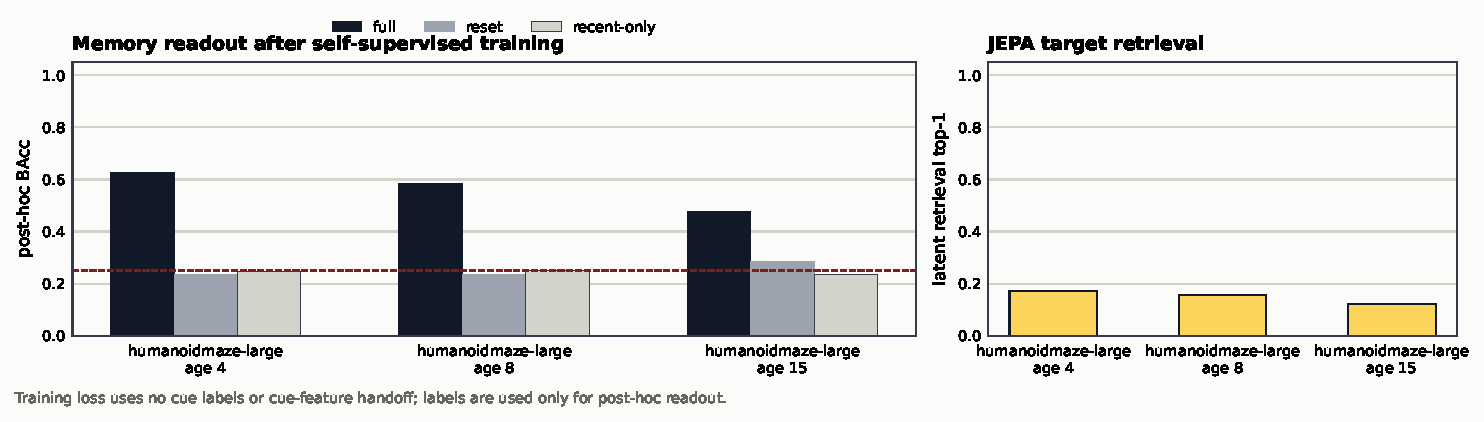
\includegraphics[width=\linewidth]{figures/fig_b_nonmanual_extra_humanoidmaze_large_navigate_v0.pdf}
\caption{Generated non-manual breadth plot for humanoidmaze-large-navigate-v0.}
\end{figure}

\begin{table}[!tbp]
\centering
\scriptsize
\setlength{\tabcolsep}{3.5pt}
\renewcommand{\arraystretch}{1.05}
\caption{Generated non-manual breadth table for humanoidmaze-large-navigate-v0.}
\begin{tabular}{lccccccl}
\toprule
Deck & Age & Seeds & Pass & Full & Reset & Recent & Status\\
\midrule
humanoidmaze-large-navigate-v0 & 4 & 3 & 1/3 & 0.626 & 0.234 & 0.247 & \textsc{mixed}\\
humanoidmaze-large-navigate-v0 & 8 & 3 & 0/3 & 0.585 & 0.236 & 0.250 & \textsc{mixed}\\
humanoidmaze-large-navigate-v0 & 15 & 3 & 0/3 & 0.476 & 0.285 & 0.236 & \textsc{mixed}\\
\bottomrule
\end{tabular}
\end{table}



\section{Detailed claim ledger}

\begin{table}[H]
\centering
\footnotesize
\caption{Expanded ledger corresponding to Figure~\ref{fig:claim-ledger}.  The
main paper uses the visual ledger; this table records the detailed boundary for
each row.}
\begin{tabularx}{\linewidth}{lYcccY}
\toprule
Environment & Host / task & Retention & Exposure & Use & Boundary\\
\midrule
PushT & DINO-WM and LeWM, six-way visual binding, age 15
  & \Pass & \Pass & \Pass
  & Cross-host use gate passes; host-native banks prevent a row-matched causal
    comparison between host families.\\
PointMaze & DINO-WM, four-goal transient cue
  & \Pass & \Pass & \Pass
  & Strong external consumer result; not native planner memory.\\
Wall & DINO-WM, four-position transient wall cue
  & \Pass & mixed & \NA
  & Carrier-prior memory remains high; host-output exposure confirms only at
    short cue age.\\
OGBench & Seven admitted decks; repaired fixed-controller native use plus
  two-deck non-manual patch-set JEPA
  & \Pass & \Pass & \Pass
  & Admission passes across seven decks.  The repaired native-use sweep scores
    24/36 env-age rows under fixed controllers, and the non-manual patch-set
    JEPA stage passes all 30 registered PointMaze-large/Cube-single retention
    cells.  No native OGBench planner is claimed.\\
\bottomrule
\end{tabularx}
\end{table}

\section{Quantitative result summary}

\paragraph{PushT checkpointed use.}
At age 15, both frozen host families support the same qualitative conclusion:
full memory separates from reset and no-state controls in host readout and
executed success.  DINO-WM full memory reaches balanced accuracy 0.988 and
executed success 0.972, while reset/no-state execution remains near the
six-way uninformed regime.  LeWM full memory reaches balanced accuracy 0.920
and executed success 0.926 with the same control pattern.

\begin{table}[H]
\centering
\footnotesize
\caption{PushT binding use summary.}
\begin{tabular}{lccc}
\toprule
Host & Full execution & Reset execution & No-state execution\\
\midrule
DINO-WM & 0.972 & 0.167 & 0.168\\
LeWM    & 0.926 & 0.156 & 0.151\\
\bottomrule
\end{tabular}
\end{table}

\paragraph{PointMaze external use.}
The fixed consumer preserves the carrier ordering in navigation execution.  No
state remains close to random-goal behavior; state-space and fixed-trust are
the strongest arms.

\begin{table}[H]
\centering
\footnotesize
\caption{PointMaze external-use summary.}
\begin{tabular}{lcc}
\toprule
Arm & Goal/read accuracy & Executed success\\
\midrule
No state & 0.250 & 0.239\\
GRU & --- & 0.302\\
LSTM & --- & 0.484\\
State-space & 0.760 & 0.745\\
Fixed-trust & 0.866 & 0.775\\
\bottomrule
\end{tabular}
\end{table}

\paragraph{Wall readout note.}
The Wall carrier grid was first screened with a deterministic ridge readout.
That screen suggested fixed-trust might clear host-output exposure at ages 4
and 8.  The paper uses the stricter confirmation run instead:
StandardScaler, PCA(256), and logistic regression fit only on the training
split.  Under this confirmation fixed-trust clears only age 4, while
state-space does not clear any age.  This is why Wall is described as exposure
failure localization rather than a broad success result.

\begin{table}[H]
\centering
\footnotesize
\caption{Wall confirmation: carrier prior remains high while host-output
exposure decays.}
\begin{tabular}{llccc}
\toprule
Arm & Readout & Age 4 & Age 8 & Age 15\\
\midrule
Fixed-trust & carrier prior & 1.000 & 1.000 & 1.000\\
Fixed-trust & host output & 0.929 & 0.446 & 0.297\\
State-space & carrier prior & 1.000 & 0.995 & 0.989\\
State-space & host output & 0.565 & 0.301 & 0.272\\
\bottomrule
\end{tabular}
\end{table}

\section{OGBench claim boundary}

The OGBench admission bridge checks only whether a controlled cue deck is
valid: cue-time encoding must be high, endpoint/action/state shortcuts must be
near chance, and counterfactual masks must not leak post-cue evidence.  It
does not train a frozen OGBench world model and does not run downstream
execution.

The follow-up feature-host stage is one rung stronger but still bounded.  It
uses admitted decks, DINOv2 pooled patch features as a frozen feature
interface, and a sidecar that carries the old cue feature before writing a
residual into the endpoint feature.  The writer loss is self-supervised against
the cue feature, while labels are used only for the post-hoc readout.

The native-use stage then asks whether the selected label changes final
environment success.  Non-teleport PointMaze uses a BFS waypoint controller
over native point-mass actions.  Cube variants use the OGBench
CubeMarkovOracle with selected-label target metadata, Puzzle uses a lights-out
solve with the button oracle, and Scene composes button, drawer, window, and
cube Markov oracles.  The repaired sweep scores 24/36 env-age rows; the
PointMaze-teleport controller gate remains below threshold, and
AntMaze/HumanoidMaze remain unscored without local low-level controllers.
These are fixed-controller use checks; they are not native OGBench world-model
planning.

The final non-manual stage then removes the explicit cue-feature handoff on
PointMaze-large and Cube-single.  It mines salient target frames and patch
sets without cue labels or cue-layout knowledge, predicts fixed generic
color/texture patch latents through compact slots, and evaluates the learned
state only after training.  This certifies autonomous old-evidence retention
for the two core render-stage decks, but not yet broad OGBench-wide
generalization or native planner memory.

\begin{table}[H]
\centering
\footnotesize
\caption{OGBench admission summary.  All rows pass cue-time readability,
shortcut, and mask checks; all memory/use columns are intentionally unclaimed.}
\begin{tabularx}{\linewidth}{lYccc}
\toprule
Deck & Family & Cue read & Max shortcut & Mask audit\\
\midrule
PointMaze-large-navigate & navigation & 1.000 & 0.250 & pass\\
AntMaze-large-navigate & locomotion & 1.000 & 0.250 & pass\\
HumanoidMaze-large-navigate & high-DoF locomotion & 1.000 & 0.250 & pass\\
Cube-single-play & object manipulation & 1.000 & 0.250 & pass\\
Cube-double-play & object manipulation & 1.000 & 0.250 & pass\\
Scene-play & multi-object scene & 1.000 & 0.250 & pass\\
Puzzle-3x3-play & combinatorial puzzle & 1.000 & 0.250 & pass\\
\bottomrule
\end{tabularx}
\end{table}

\begin{table}[H]
\centering
\footnotesize
\caption{OGBench feature-host capacity summary.  Gate: full host-output
balanced accuracy at least 0.750, reset and no-state controls at most 0.300.
All rows use 200 train bases, 80 validation bases, and five seeds.}
\begin{tabular}{lcccc}
\toprule
Deck & Age & Seeds passing & Full & Reset/no-state\\
\midrule
AntMaze-large-navigate & 4  & 5/5 & 1.000 & 0.250 / 0.250\\
AntMaze-large-navigate & 8  & 5/5 & 1.000 & 0.250 / 0.250\\
AntMaze-large-navigate & 15 & 5/5 & 1.000 & 0.250 / 0.250\\
Cube-single-play       & 4  & 5/5 & 1.000 & 0.250 / 0.250\\
Cube-single-play       & 8  & 5/5 & 1.000 & 0.250 / 0.250\\
Cube-single-play       & 15 & 5/5 & 1.000 & 0.250 / 0.250\\
\bottomrule
\end{tabular}
\end{table}

Table~\ref{tab:native-use-repaired-allenv} reports the repaired all-env
native-use sweep.  It subsumes the earlier PointMaze-large/Cube-single slice
and keeps controller-gate failures and unavailable locomotion controllers as
explicit scope limits.

\begin{table}[H]
\centering
\footnotesize
\caption{Final non-manual OGBench patch-set JEPA summary.  Labels are used
only for post-hoc audit; training uses no cue labels, cue crops, or key-frame
annotations.}
\begin{tabular}{lccccc}
\toprule
Deck & Age & Seeds passing & Full & Reset & Recent-only\\
\midrule
PointMaze-large-navigate & 4  & 5/5 & 1.000 & 0.251 & 0.255\\
PointMaze-large-navigate & 8  & 5/5 & 0.994 & 0.266 & 0.250\\
PointMaze-large-navigate & 15 & 5/5 & 0.983 & 0.251 & 0.252\\
Cube-single-play         & 4  & 5/5 & 1.000 & 0.240 & 0.257\\
Cube-single-play         & 8  & 5/5 & 0.990 & 0.223 & 0.254\\
Cube-single-play         & 15 & 5/5 & 0.921 & 0.247 & 0.246\\
\bottomrule
\end{tabular}
\end{table}
